\documentclass[12pt]{article}

% Packages
\usepackage{lipsum}
\usepackage{setspace}
\usepackage{indentfirst}
\usepackage{geometry}
\usepackage[nonumberlist, toc]{glossaries}
\usepackage{graphicx}
\usepackage{caption}
\usepackage{subcaption}
\usepackage{tabularx}
\usepackage{booktabs}
\usepackage[numbered]{./latex/mcode}
\usepackage{enumitem}
\usepackage{xcolor}
\usepackage [autostyle, english = american]{csquotes}
\usepackage{fancyhdr}
\usepackage{amsmath}
\usepackage{cite}

% Formatting
\geometry{letterpaper, portrait, margin=.85in}

\pagestyle{fancy}
\lhead{MSXII Suspension Parameters}
\rhead{Midnight Sun Solar Car Team}

\MakeOuterQuote{"}

\begin{document}

% Title Ppage
\begin{titlepage}
	\vspace*{3cm}
	\centering
	
\includegraphics[width=.25\textwidth]{./LaTex/midnightSunLogoCircle.png}\par
	\vspace{1.5cm}
	{\scshape\LARGE Midnight Sun Solar Car Team \par}
	{\scshape\large University of Waterloo\par}
	\vspace{3.5cm}
	{\huge\bfseries FEA Boundary Conditions\par}
	\vspace{0.2cm}
	\large MSXII
	\vfill
	Prepared by:\par
	Devon Copeland\par
	\vspace{1cm}
	\today\par
\end{titlepage}

% Main Matter
\section{Background}
\subsection{Vehicle Design}
Midnight Sun Twelve (MSXII) is a cruiser class, solar electric vehicle being designed with the goal of competing in the 2018 American Solar Challenge (ASC 2018) and the 2019 World Solar Challenge (WSC 2019). By definition, cruiser class solar vehicles must be multi-occupant and are designed with the intent of being more practical than a typical, challenger class solar car. Because of the unique requirements of this class, the spring rates and target damping coefficients on MSXII's suspension must be selected to optimize for efficiency while still keeping driver comfort in mind. This report proposes an analytical technique for determining the response of a suspension system to any given road conditions. 

\subsection{Important Vehicle Parameters}
Table \ref{tab:params} lists vehicle parameters that are of importance to the design and analysis of MSXII's suspension. The mass and moment of inertia was computed by CAD software. 
\begin{table}[htbp]
	\centering
	\caption{Important Vehicle Parameters}
	\label{tab:params}
	\begin{tabular}{lll}
	Mass ($M$)                            	& 550  & $kg$       \\
	Wheelbase                       	 	& 2.60  & $m$  		\\
	Track                       	 		& 1.60  & $m$  		\\
	Distance from Front Wheel to CoG ($a$)	& 1.32 & $m$  		\\
	Distance from Road to CoG ($h$)		& 0.52 & $m$  		\\
	Moment of Inertia Normal to Symmetry Plane at CoG ($I_{xx}$) & 550  & $kgm^2$ \\
	Full Wheel Travel in Compression 	& 45   & $mm$ 		\\
	Front Coilover Angle from Vertical	& 40   & $\circ$ 	\\
	Rear Coilover Angle from Vertical	& 30   & $\circ$
	\end{tabular}
\end{table}
\subsection{Suspension Architecture}
MSXII's front suspension comprises of a double wishbone linkage with an outboard coilover while the rear suspension comprises of independent trailing arms allowing for zero scrub and thus less rolling resistance. Figure \ref{fig:solidworksScreenshots} shows the screenshots of the front and rear suspension.  
\begin{figure}[htbp]
	\centering
    \begin{subfigure}[b]{.32\textwidth}
		\caption{Front Isometric View}
		\centering
        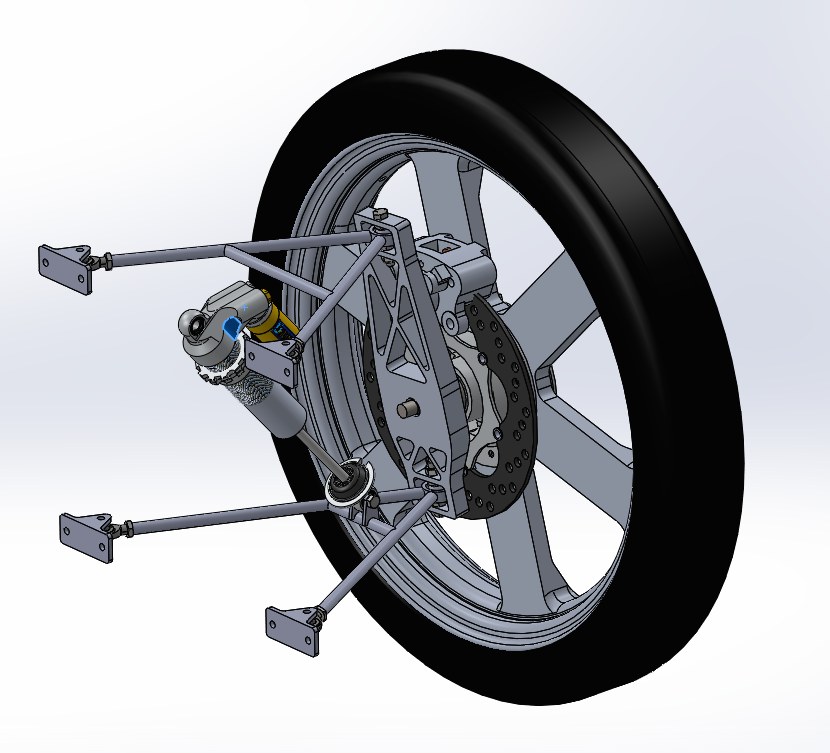
\includegraphics[height=3.5cm]{./LaTex/frontIso.PNG}
    \end{subfigure}
    \begin{subfigure}[b]{.32\textwidth}
		\caption{Rear Isometric View}
		\centering
        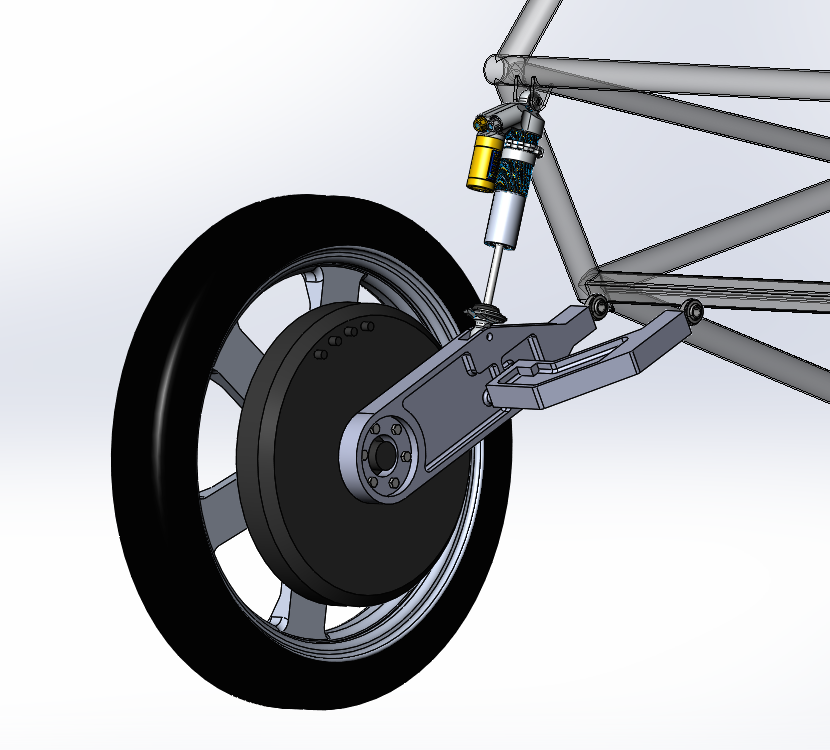
\includegraphics[height=3.5cm]{./LaTex/rearIso.PNG}
        \label{fig:c8}
    \end{subfigure}
    \begin{subfigure}[b]{.32\textwidth}
		\caption{Rear Sie View}
		\centering
        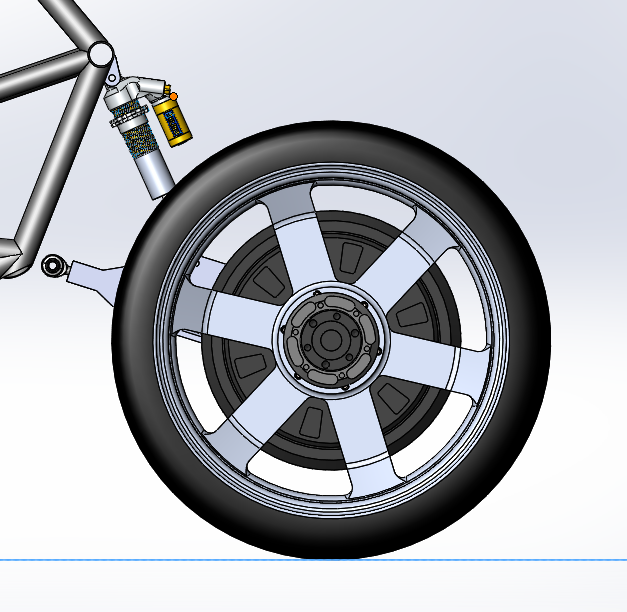
\includegraphics[height=3.5cm]{./LaTex/rearRight.PNG}
        \label{fig:c9}
    \end{subfigure}
    \caption{MSXII Suspension Design (Screenshots from Solidworks)}
	\label{fig:solidworksScreenshots}
\end{figure}
\subsection{Two Loading Conditions}
Two cases of boundary conditions are considered for FEA. One case occurs when the suspension is statically loaded during the extreme case of braking while cornering. The other case is a dynamic loading scenario where the car suddenly hits a bump at speed. 

It is important to note that the former case (that of braking while cornering) is specific to the front suspension. The equivalent worst case loading scenario for the rear would occur while accelerating during a corner. However, since MSXII's motors produce only ***Nm of torque while the brakes require ***Nm to slow the car at the required rate, the worst loading for the front will far exceed that of the rear. For simplicity, this value is treated as the worst case for both the front and the rear. 

\section{Static Loading}
\label{sec:paramSelection}
Assuming a smooth driving surface, the largest normal force acting on the tire will occur while braking in a turn. To approximate this loading condition, the a superposition of two static half car models is used; one for cornering and one for hard braking.  
\subsubsection{Hard Braking}\begin{figure}[h!]
	\centering
	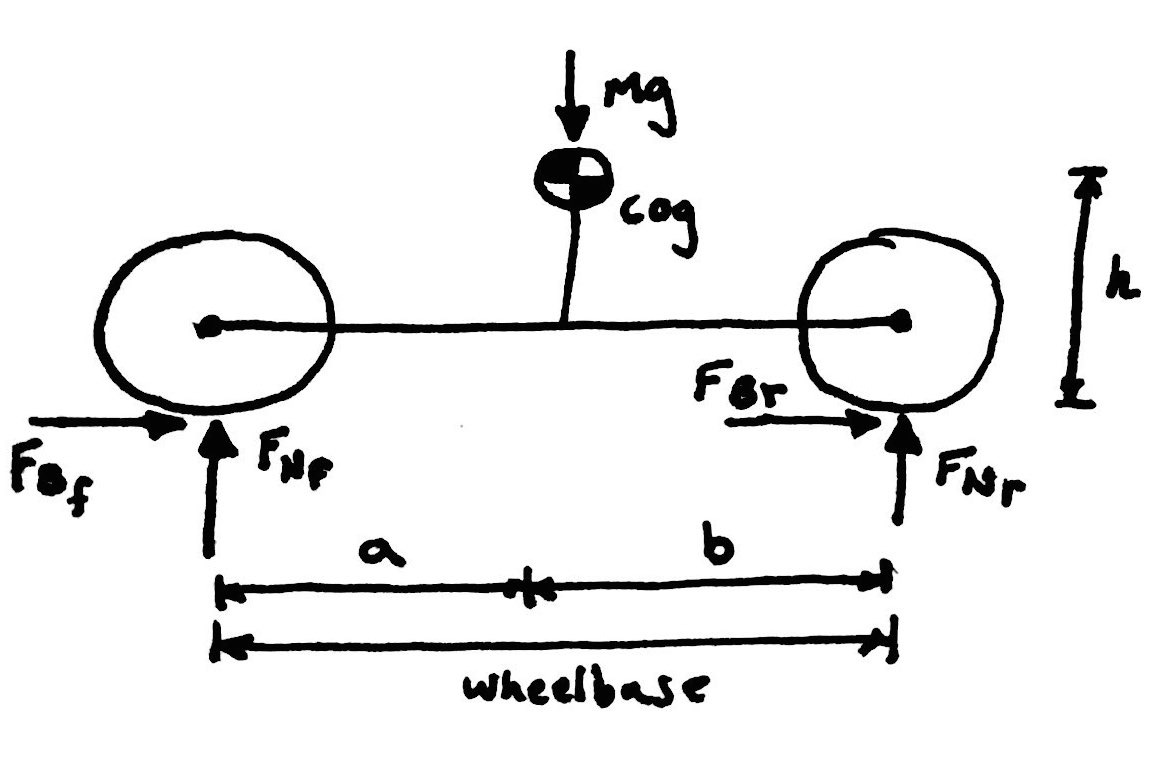
\includegraphics[width=.5\textwidth]{./LaTex/brakingFBD.jpg}
	\caption{Free Body Diagram of a Car Braking}
	\label{fig:barkingFBD}
\end{figure}
Figure \ref{fig:barkingFBD} shows a free body diagram of a half car model undergoing braking. MSXII will only have brake callipers on the front wheels however regenerative braking from the hub motors will also provide a braking force at the rear contact patches. Assuming a generous coefficient of static friction, $\mu _s$, of 1.0 and the extreme case where the both the font and rear tires are about to begin sliding, the combined braking force can be expressed as: 
\begin{equation}
	F_{braking} = F_{Nf} + F_{Nr} = \mu _s F_{N_{net}} =  \mu _s Mg = (1.0)(550kg)\left(9.81\frac{m}{s^2}\right) = 5.40kN
\end{equation}
From Figure \ref{fig:barkingFBD}, summing the moments about the centre of gravity and the vertical forces results in the following equations: 
\begin{equation}
	aF_{Nf} = hF_{braking} + bF_{Nr}
\end{equation}
\begin{equation}
	F_{Nf} + F_{Nr} = Mg
\end{equation}
Solving for the front normal force: 
\begin{equation}
\begin{split}
	aF_{Nf} &= hF_{braking} + b(Mg - F_{Nf})\\
	F_{Nf} &= \frac{hF_{braking} + bMg}{a+b} = \frac{(0.52m)(5.40kN)+(1.28m)(550kg)\left(9.81\frac{m}{s^2}\right)}{(1.32m)+(1.28m)} = 3.74kN
\end{split}
\end{equation}
Note that 3.74kN is for both front wheels. Therefore there is approximately \textbf{1.87kN} of normal force on each front tire during hard braking. 

\subsubsection{Cornering}
\begin{figure}[h!]
	\centering
	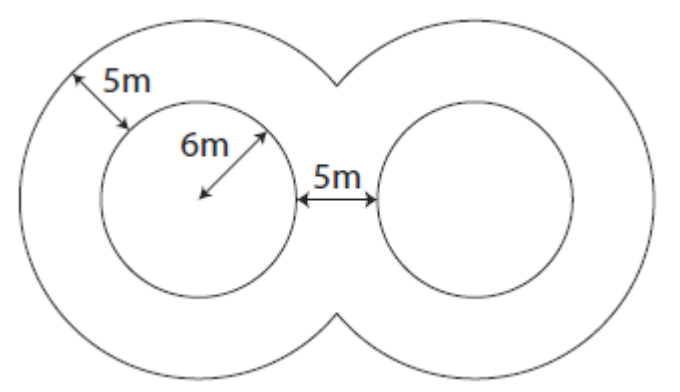
\includegraphics[width=.5\textwidth]{./LaTex/dynamicScrutineering.PNG}
	\caption{Figure of Eight Course from ASC 2018 Regulations 
	\cite{ASC2018regs}}
	\label{fig:dynamicScrutineering}
\end{figure}
The ASC 2018 regulations stipulate that a vehicle must be able to navigate a figure of eight as shown in Figure \ref{fig:dynamicScrutineering} in less than 18 seconds \cite{ASC2018regs}. Since the average arc length of the figure of eight is $34\pi m$, the net cornering force required to navigate the figure of eight can be found as follows:
\begin{equation}
	F_{si} + F_{so} = F_{steer} = \frac{Mv^2}{r} = \frac{(550kg)\left(\frac{34\pi m}{18s}\right)^2}{8.5m} = 2.28kN
\end{equation}
\begin{figure}[h!]
	\centering
	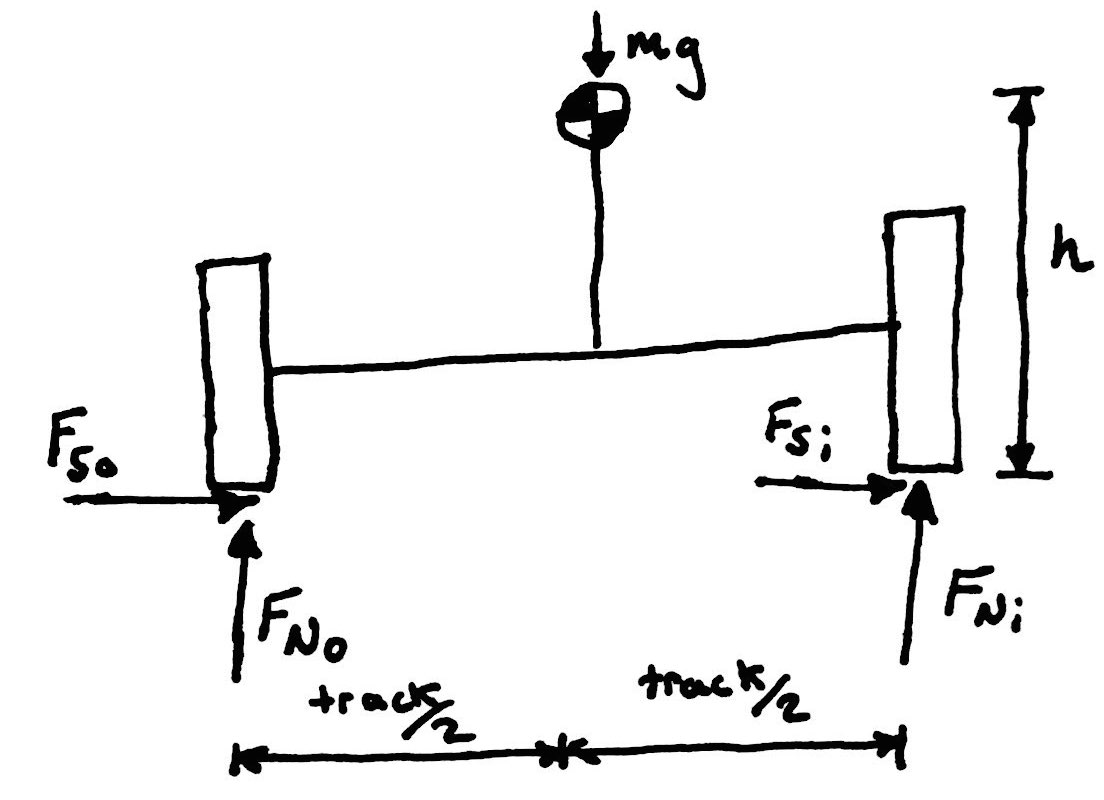
\includegraphics[width=.5\textwidth]{./LaTex/steerFBD.jpg}
	\caption{Free Body Diagram of a Car Cornering}
	\label{fig:steerFBD}
\end{figure}

\noindent For the half car model shown if Figure \ref{fig:steerFBD}, summing the moments about the centre of gravity and the vertical forces results in the following equations: 
\begin{equation}
	\frac{track}{2}F_{No} = hF_{steer} + \frac{track}{2}F_{Ni}
\end{equation}
\begin{equation}
	F_{No} + F_{Ni} = Mg
\end{equation}
Solving for the outside wheel normal force: 
\begin{equation}
\begin{split}
	\frac{track}{2}F_{No} &= hF_{steer} + \frac{track}{2}(Mg - F_{Ni})\\
	F_{No} &= \frac{hF_{steer} + \frac{track}{2}Mg}{track} = \frac{(0.52m)(2.28kN)+(0.80m)(550kg)\left(9.81\frac{m}{s^2}\right)}{1.60m} = 3.44kN
\end{split}
\end{equation}
Note that the 3.44kN above is for both front and rear outside wheels. Assuming the force is evenly split between the front and rear, there is approximately \textbf{1.72kN} of normal force on each outside tire during maximum cornering. 
\subsubsection{Superposition}
Both the braking and cornering conditions subject the front outside wheel to a normal force greater than the nominal normal force seen when the car is at rest. The change in normal force for each loading condition can be expressed as follows: 
\begin{equation}
	\begin{split}
		\Delta F_{N_{braking}} &= F_{Nf_{braking}} - \frac{Mg}{4} =  1.87kN - 1.35kN = 0.52kN\\
		\Delta F_{N_{cornering}} &=  F_{No_{cornering}} - \frac{Mg}{4} =  1.72kN - 1.35kN = 0.37kN
	\end{split}
\end{equation}
To approximate the worst case loading condition, a superposition of the changes in normal force and the nominal normal force is applied. 
\begin{equation}
	F_{N_{max}} = \Delta F_{N_{braking}} + \Delta F_{N_{cornering}} + F_{N_{nominal}} = 0.52kN + 0.37kN + 1.35kN = 2.24kN
\end{equation}

\section{Dynamic Loading}
MSXII will be using Ohlins TTX25 dampers for both the front and rear suspension. From the Ohlins' published data, \cite{tbd}, the maximum damping coefficient achievable is approximately 3.5kNs/m. 

% Source
\pagebreak
\bibliography{bib}{}
\bibliographystyle{plain}

% Appendix
\pagebreak
\appendix
\section{MATLAB Source Code for Simplified Model}
\label{app:simple}
\lstinputlisting[breaklines=true]{./matlab/alternativeFormulation.m}
\pagebreak
\section{MATLAB Source Code for Alternative Formulation}
\label{app:alternative}
\lstinputlisting[breaklines=true]{./matlab/simplifiedFormulation.m}

\end{document}